\documentclass[tikz,border=8pt]{standalone}
% Shared look for every TikZ diagram. Load with \input{../../tools/tikz-style.tex}
\usepackage[T1]{fontenc}
\usepackage{lmodern}
\renewcommand{\sfdefault}{lmr}  % diagrams use the same serif as the text
\usetikzlibrary{arrows.meta, positioning, shapes.geometric, calc, fit, backgrounds}
\definecolor{cblue}{HTML}{4C78A8}
\definecolor{corange}{HTML}{F58518}
\definecolor{cgreen}{HTML}{54A24B}
\definecolor{cred}{HTML}{E45756}
\definecolor{cpurple}{HTML}{B279A2}
\definecolor{cgrey}{HTML}{6B6B6B}
\tikzset{
  every picture/.style={font=\sffamily, line width=1.2pt},
  box/.style={draw=#1, fill=#1!12, rounded corners=4pt, align=center, inner sep=7pt, minimum height=1.1cm},
  box/.default=cgrey,
  arrow/.style={-{Stealth[length=3mm]}, draw=cgrey, line width=1.4pt},
  title/.style={font=\sffamily\bfseries\Large},
  note/.style={font=\sffamily\small, text=cgrey, align=center},
}
\AtBeginDocument{\hyphenpenalty=10000 \exhyphenpenalty=10000}

\begin{document}
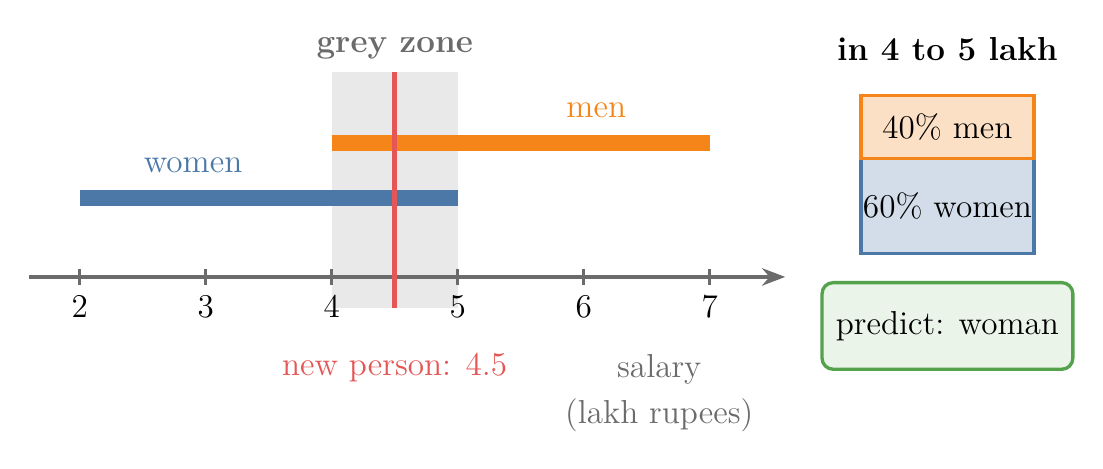
\begin{tikzpicture}[every node/.append style={font=\sffamily\large}, x=1.6cm]
  \fill[cgrey!15] (4,-0.4) rectangle (5,2.6);
  \node[text=cgrey, font=\sffamily\large\bfseries] at (4.5,2.9) {grey zone};
  \draw[cgrey, -{Stealth}] (1.6,0) -- (7.6,0) ;
  \foreach \v in {2,...,7} {\draw[cgrey] (\v,-0.1) -- (\v,0.1); \node[below=3pt] at (\v,0) {\v};}
  \draw[cblue, line width=6pt] (2,1.0) -- (5,1.0) node[pos=0.3, above=3pt, text=cblue] {women};
  \draw[corange, line width=6pt] (4,1.7) -- (7,1.7) node[pos=0.7, above=3pt, text=corange] {men};
  \draw[cred, line width=1.6pt] (4.5,-0.4) -- (4.5,2.6);
  \node[text=cred, below=24pt] at (4.5,0) {new person: 4.5};
  \node[text=cgrey, below=24pt] at (6.6,0) {salary};
  \node[text=cgrey, below=40pt] at (6.6,0) {(lakh rupees)};
  % share bar in the zone
  \begin{scope}[shift={(8.2,0.3)}, x=1cm]
    \node[font=\sffamily\large\bfseries] at (1.1,2.6) {in 4 to 5 lakh};
    \draw[draw=cblue, fill=cblue!25] (0,0) rectangle (2.2,1.2) node[midway] {60\% women};
    \draw[draw=corange, fill=corange!25] (0,1.2) rectangle (2.2,2.0) node[midway] {40\% men};
    \node[box=cgreen, below=10pt, inner sep=5pt] at (1.1,0) {predict: woman};
  \end{scope}
\end{tikzpicture}
\end{document}
